%%% Compiled with XeLaTeX
%%% Generate the GIF with convert -delay 100 -loop 0 -density 200 -alpha on 
%%% file.pdf file.gif (package imagemagick is required)
\documentclass[tikz,border=10pt]{standalone}
% \usepackage{fontspec}
% \setmainfont{Roboto Light}
\usepackage{pgfplots}
\pgfplotsset{compat=newest}

\definecolor{myblue}{RGB}{25,130,196}
\definecolor{myblue2}{RGB}{25,50,220}
\definecolor{mygreen}{RGB}{100,180,28}
\definecolor{myyellow}{RGB}{255,202,58}
\definecolor{myorange}{RGB}{255,154,92}
\definecolor{myred}{RGB}{255,92,97}
\definecolor{mypurple}{RGB}{116,83,162}
\definecolor{fg}{RGB}{150,150,150}
\definecolor{mygray}{RGB}{190,190,190}

\colorlet{myblue-mild}{myblue!60}
\colorlet{myblue2-mild}{myblue2!60}
\colorlet{mygreen-mild}{mygreen!60}
\colorlet{myyellow-mild}{myyellow!60}
\colorlet{myorange-mild}{myorange!60}
\colorlet{myred-mild}{myred!60}
\colorlet{mypurple-mild}{mypurple!60}
\colorlet{mygray-mild}{mygray!60}


\pgfplotstableread[col sep=comma]{data.csv}{\data}

\begin{document}

\newcommand{\plota}{
    \addplot[mark=*,solid,every mark/.append style={solid,fill=mypurple, 
             fill opacity=0.2},color=mypurple,very thick,mark size=4pt]
        table[x=ka,y=lu] {\data}; 


    \addplot[mark=x,solid,every mark/.append style={solid,fill=mygray, 
             fill opacity=0.},color=mygray,opacity=0.,very thick,mark size=4pt,
             empty legend] 
         table[x=ka,y=ds] {\data};    


    \addplot[mark=triangle*,solid,every mark/.append style={solid, fill=mygray,
             fill opacity=0.},color=mygray,opacity=0.,very thick,mark size=4pt,
             empty legend] 
         table[x=ka,y=dd] {\data};    


    \addplot[mark=square*,solid,every mark/.append style={solid, fill=mygray, 
             fill opacity=0.},color=mygray,opacity=0.,very thick,mark size=4pt,
             empty legend] 
         table[x=ka,y=dq] {\data};    

    \legend{LU-IR, \phantom{$u_{p}=$ \textsc{s}}, \phantom{$u_{p}=$
            \textsc{d}}, \phantom{$u_{p}=$ \textsc{q}}, }
}
\newcommand{\plotb}{
    \addplot[mark=*,solid,every mark/.append style={solid,fill=mypurple, 
             fill opacity=0.2},color=mypurple,very thick,mark size=4pt] 
        table[x=ka,y=lu] {\data}; 


    \addplot[mark=x,solid,every mark/.append style={solid,fill=mygray, 
             fill opacity=0.},color=mygray,opacity=0.,very thick,mark size=4pt,
             empty legend] 
         table[x=ka,y=ds] {\data};    


    \addplot[mark=triangle*,solid,every mark/.append style={solid, fill=mygray,
             fill opacity=0.},color=mygray,opacity=0.,very thick,mark size=4pt,
             empty legend] 
         table[x=ka,y=dd] {\data};    


    \addplot[mark=square*,solid,every mark/.append style={solid, fill=myred, 
             fill opacity=0.2},color=myred,very thick,mark size=4pt] 
         table[x=ka,y=dq] {\data};    

    \legend{LU-IR, \phantom{$u_{p}=$ \textsc{s}}, \phantom{$u_{p}=$ 
            \textsc{d}}, $u_{p}=$ \textsc{q}, }
}
\newcommand{\plotc}{
    \addplot[mark=*,solid,every mark/.append style={solid,fill=mypurple, 
             fill opacity=0.2},color=mypurple,very thick,mark size=4pt] 
        table[x=ka,y=lu] {\data}; 


    \addplot[mark=x,solid,every mark/.append style={solid,fill=mygray, 
             fill opacity=0.},color=mygray,opacity=0.,very thick,mark size=4pt,
             empty legend] 
         table[x=ka,y=ds] {\data};    


    \addplot[mark=triangle*,solid,every mark/.append style={solid, 
             fill=mygreen, fill opacity=0.2},color=mygreen,very thick,
             mark size=4pt] 
         table[x=ka,y=dd] {\data};    


    \addplot[mark=square*,solid,every mark/.append style={solid, fill=myred, 
             fill opacity=0.2},color=myred,very thick,mark size=4pt] 
         table[x=ka,y=dq] {\data};    

    \legend{LU-IR, \phantom{$u_{p}=$ \textsc{s}}, $u_{p}=$ \textsc{d}, 
            $u_{p}=$ \textsc{q}, }
}
\newcommand{\plotd}{
    \addplot[mark=*,solid,every mark/.append style={solid,fill=mypurple, 
             fill opacity=0.2},color=mypurple,very thick,mark size=4pt] 
        table[x=ka,y=lu] {\data}; 


    \addplot[mark=x,solid,every mark/.append style={solid,fill=myyellow,
             fill opacity=0.2},color=myyellow,very thick,mark size=4pt] 
         table[x=ka,y=ds] {\data};    


    \addplot[mark=triangle*,solid,every mark/.append style={solid,
             fill=mygreen, fill opacity=0.2},color=mygreen,very thick,
             mark size=4pt] 
         table[x=ka,y=dd] {\data};    


    \addplot[mark=square*,solid,every mark/.append style={solid, fill=myred,
             fill opacity=0.2},color=myred,very thick,mark size=4pt] 
         table[x=ka,y=dq] {\data};    

    \legend{LU-IR, $u_{p}=$ \textsc{s}, $u_{p}=$ \textsc{d}, $u_{p}=$ 
            \textsc{q}, }
}

\foreach \whichplot in {\plota,\plotb,\plotc,\plotd}
{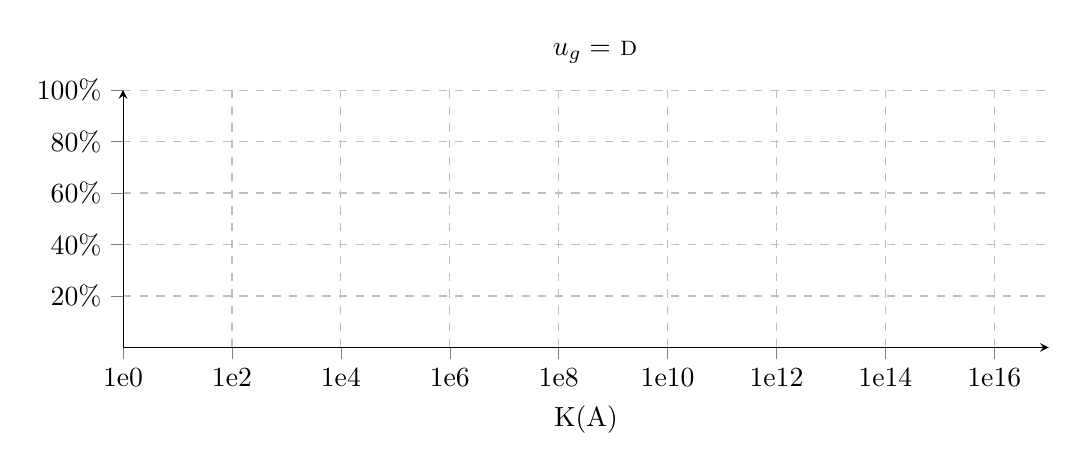
\begin{tikzpicture}
    \begin{axis}
    [
        legend style={at={(0.195,0.65)}, font=\scriptsize},
        axis x line=left,
        axis y line=middle,
        grid = major,
        width=1.1\linewidth,
        height=0.4\linewidth,
        grid style={dashed, gray!50},
        xmin= 1e0,
        xmax= 1e17,
        xmode=log,
        xtick={1e0, 1e2, 1e4, 1e6, 1e8, 1e10, 1e12, 1e14, 1e16},
        xticklabels={1e0, 1e2, 1e4, 1e6, 1e8, 1e10, 1e12, 1e14, 1e16},
        ymin= 0.,
        ymax= 1.,
        ytick={0.2, 0.4, 0.6, 0.8, 1},
        yticklabels={20\%, 40\%, 60\%, 80\%, 100\%},
        xlabel=K(A),
        tick align=outside,
        enlargelimits=false,
        title={\phantom{$S$}$u_g=$ \textsc{d}}
    ]

    \whichplot

\end{axis}
\end{tikzpicture}}

\begin{tikzpicture}
    \begin{axis}
    [
        legend style={at={(0.195,0.65)}, font=\scriptsize},
        axis x line=left,
        axis y line=middle,
        grid = major,
        width=1.1\linewidth,
        height=0.4\linewidth,
        grid style={dashed, gray!50},
        xmin= 1e0,
        xmax= 1e17,
        xmode=log,
        xtick={1e0, 1e2, 1e4, 1e6, 1e8, 1e10, 1e12, 1e14, 1e16},
        xticklabels={1e0, 1e2, 1e4, 1e6, 1e8, 1e10, 1e12, 1e14, 1e16},
        ymin= 0.,
        ymax= 1.,
        ytick={0.2, 0.4, 0.6, 0.8, 1},
        yticklabels={20\%, 40\%, 60\%, 80\%, 100\%},
        xlabel=K(A),
        tick align=outside,
        enlargelimits=false,
        title={\phantom{$S$}$u_g=$ \textsc{s}}
    ]

        \addplot[mark=*,solid,every mark/.append style={solid, fill=mypurple, 
                 fill opacity=0.2},color=mypurple,very thick,mark size=4pt] 
            table[x=ka,y=lu] {\data};    

        \addplot[mark=x,solid,every mark/.append style={solid, fill=myyellow,
                 fill opacity=0.2},color=myyellow,very thick,mark size=4pt] 
             table[x=ka,y=ss] {\data};    

        \addplot[mark=triangle*,solid,every mark/.append style={solid, 
                 fill=mygreen, fill opacity=0.2},color=mygreen,very thick,
                 mark size=4pt] 
             table[x=ka,y=sd] {\data};

        \addplot[mark=square*,solid,every mark/.append style={solid, 
                 fill=myred, fill opacity=0.2},color=myred,very thick,
                 mark size=4pt] 
             table[x=ka,y=sq] {\data};    

        \addplot[mark=x,solid,every mark/.append style={solid,fill=mygray, 
                 fill opacity=0.},color=gray,draw opacity = 0.3,very thick,
                 mark size=4pt,forget plot] 
             table[x=ka,y=ds] {\data};    

        \addplot[mark=triangle*,solid,every mark/.append style={solid, 
                 fill=mygray, fill opacity=0.},color=gray,draw opacity = 0.3,
                 very thick,mark size=4pt,forget plot] 
             table[x=ka,y=dd] {\data};    

        \addplot[mark=square*,solid,every mark/.append style={solid, 
                 fill=mygray, fill opacity=0.},color=gray,draw opacity = 0.3,
                 very thick,mark size=4pt,forget plot] 
             table[x=ka,y=dq] {\data};

            \legend{LU-IR, $u_p=$ \textsc{s}, $u_p=$ \textsc{d}, $u_p=$
                    \textsc{q}}
    \end{axis}
\end{tikzpicture}

\begin{tikzpicture}
    \begin{axis}
    [
        legend style={at={(0.195,0.65)}, font=\scriptsize},
        axis x line=left,
        axis y line=middle,
        grid = major,
        width=1.1\linewidth,
        height=0.4\linewidth,
        grid style={dashed, gray!50},
        xmin= 1e0,
        xmax= 1e17,
        xmode=log,
        xtick={1e0, 1e2, 1e4, 1e6, 1e8, 1e10, 1e12, 1e14, 1e16},
        xticklabels={1e0, 1e2, 1e4, 1e6, 1e8, 1e10, 1e12, 1e14, 1e16},
        ymin= 0.,
        ymax= 1.,
        ytick={0.2, 0.4, 0.6, 0.8, 1},
        yticklabels={20\%, 40\%, 60\%, 80\%, 100\%},
        xlabel=K(A),
        tick align=outside,
        enlargelimits=false,
        title={\phantom{$S$}$u_g=$ \textsc{h}}
    ]

        \addplot[mark=*,solid,every mark/.append style={solid, fill=mypurple,
                 fill opacity=0.2},color=mypurple,very thick,mark size=4pt] 
            table[x=ka,y=lu] {\data};    

        \addplot[mark=x,solid,every mark/.append style={solid, fill=myyellow, 
                 fill opacity=0.2},color=myyellow,very thick,mark size=4pt] 
             table[x=ka,y=hs] {\data};    

        \addplot[mark=triangle*,solid,every mark/.append style={solid, 
                 fill=mygreen, fill opacity=0.2},color=mygreen,very thick,
                 mark size=4pt] 
             table[x=ka,y=hd] {\data};

        \addplot[mark=square*,solid,every mark/.append style={solid, 
                 fill=myred, fill opacity=0.2},color=myred,very thick,
                 mark size=4pt] 
             table[x=ka,y=hq] {\data};    

        \addplot[mark=x,solid,every mark/.append style={solid,fill=mygray, 
                 fill opacity=0.},color=gray,draw opacity = 0.3,very thick,
                 mark size=4pt,forget plot] 
             table[x=ka,y=ds] {\data};    

        \addplot[mark=triangle*,solid,every mark/.append style={solid,
                 fill=mygray, fill opacity=0.},color=gray,draw opacity = 0.3,
                 very thick,mark size=4pt,forget plot] 
             table[x=ka,y=dd] {\data};    

        \addplot[mark=square*,solid,every mark/.append style={solid,
                 fill=mygray, fill opacity=0.},color=gray,draw opacity = 0.3,
                 very thick,mark size=4pt,forget plot] 
             table[x=ka,y=dq] {\data};

            \legend{LU-IR, $u_p=$ \textsc{s}, $u_p=$ \textsc{d}, $u_p=$
                    \textsc{q}}
    \end{axis}
\end{tikzpicture}

\end{document}
